\documentclass{article}

% if you need to pass options to natbib, use, e.g.:
%     \PassOptionsToPackage{numbers, compress}{natbib}
% before loading neurips_2021

% ready for submission
\usepackage[preprint]{neurips_2021}

% to compile a preprint version, e.g., for submission to arXiv, add add the
% [preprint] option:
%     \usepackage[preprint]{neurips_2021}

% to compile a camera-ready version, add the [final] option, e.g.:
%     \usepackage[final]{neurips_2021}

% to avoid loading the natbib package, add option nonatbib:
%    \usepackage[nonatbib]{neurips_2021}

\usepackage[utf8]{inputenc} % allow utf-8 input
\usepackage[T1]{fontenc}    % use 8-bit T1 fonts
\usepackage[colorlinks=true]{hyperref}       % hyperlinks
\usepackage{url}            % simple URL typesetting
\usepackage{booktabs}       % professional-quality tables
\usepackage{amsfonts}       % blackboard math symbols
\usepackage{nicefrac}       % compact symbols for 1/2, etc.
\usepackage{microtype}      % microtypography
\usepackage{xcolor}         % colors

\usepackage{floatrow}
% Table float box with bottom caption, box width adjusted to content
\newfloatcommand{capbtabbox}{table}[][\FBwidth]

\usepackage{wasysym}
\usepackage{graphicx}

\usepackage{ragged2e}

\title{What attributes influence the selection of a partner?}

% The \author macro works with any number of authors. There are two commands
% used to separate the names and addresses of multiple authors: \And and \AND.
%
% Using \And between authors leaves it to LaTeX to determine where to break the
% lines. Using \AND forces a line break at that point. So, if LaTeX puts 3 of 4
% authors names on the first line, and the last on the second line, try using
% \AND instead of \And before the third author name.

\author{%
  Dustin Theobald\\
  Matrikelnummer 5967780\\
  \texttt{dustin.theobald@student.uni-tuebingen.de} \\
  \And
  Harald Kugler\\
  Matrikelnummer 4258298\\
  \texttt{harald.kugler@student.uni-tuebingen.de} \\
  \And
  Github Repository\\
  Code Documentation\\
  \texttt{\href{https://github.com/dtheo91/DataLiteracyPractical}{Project Repository}}
}

\begin{document}

\maketitle

\begin{abstract}
   We are planning to use a dataset compiled by Columbia Business School professors Ray Fisman and Sheena Iyengar: \href{https://www.kaggle.com/annavictoria/speed-dating-experiment/home?select=Speed+Dating+Data.csv}{"Evidence From a Speed Dating Experiment"} to see how well we can predict a successful first impression from several reported features, including attractiveness, sincerity, intelligence, fun, ambition, and shared interests. We are planning to compare different classifiers to logistic regression.
\end{abstract}

%You can find a detailed example and instructions on how to use this style file in the attached \texttt{neurip\_2021.tex} file. This includes instructions for how to lay out citations.
\section{Introduction}
What influences a successful first impression? How do men in women differ based on interest or rejection? This report tries to cover those questions by giving a short explanation of the exhaustive dataset, followed by a short data exploration focusing on interest overlap and the rejection between men and women. Finally it focuses on analyzing the predictive features of a successful first impression. 

\section{Dataset}
Data \cite{fisman2006gender} was gathered in 21 waves from 552 participants in experimental speed dating events from October 16th, 2002 to April 7th, 2004 in the United States compiled by Columbia Business School professors Ray Fisman and Sheena Iyenga \cite{speeddata}.
The authors generated random matching of subjects and random variation in the number of potential partners. Their design allowed them to directly observe individual decisions rather than just final matches.

During the events, the attendees would have a four minute "first date" with every other participant of the opposite sex.
At the end of their four minutes, participants were asked if they would like to see their date again. 
They were asked to rate their date on multiple attributes including
attractiveness,
sincerity,
intelligence,
fun,
ambition and
shared interests.
The dataset also contains questionnaire data gathered from participants at different points in the process. These fields include:
demographics,
dating habits,
self-perception across key attributes,
beliefs on what others find valuable in a potential partner
as well as lifestyle information.

The dataset consists of 8378 examples and 195 columns based on 278 men and 274 women with multiple partner matches per speed-dating event. Overall, 4189 dates were evaluated. The mean age of the participants is $~26.3$ with the lowest and highest age being 18, 55 and most of the participants being in their early/mid twenties to early thirties. Only $16\%$ of speed-dates were actually matches, i.e. speed-dates where both participants agreed for a follow-up date. In the following chapters we include a separate data description part as we use different features for each analysis with a separate handling of the data.

\section{Differences betweeen Men and Women}
%This chapter focuses on investigating distribution overlaps and distinction of various interests between men and women. Thereafter, we are analyzing the rejection between genders to analyze if one gender is more selective in their choice, how many positive responses were unrequited or if we are able to find rejection-patterns by showing attribute-distributions of rejected/non-rejected participants. 
\subsection{Interest Overlap and Distinction}
In this subsection we are focusing on the intersections and distinctions on multiple reported interest categories between men and women. 

\textbf{Data Preparation.} We are using six activities, which participants rated from 1 (great) to 10 (awful) in interest: Shopping, yoga, theater, dining, clubbing and movies. 
After extracting those from the raw dataset, rows including missing values as well as outliers (rating $>10$) are deleted with 8170 examples left.
We then split the data according to the genders having 4078 and 4092 examples for women and men, respectively.
\autoref{fig:interest} shows the overlaps as well as distinction in interests between men and women.

\begin{figure}[ht]
\centering
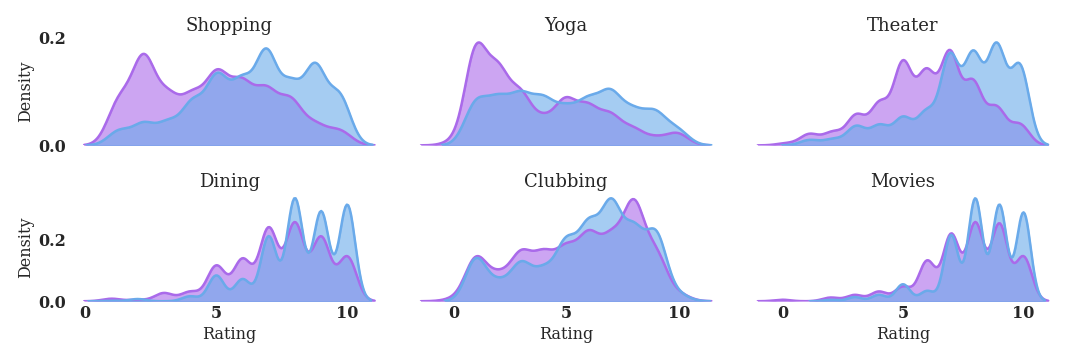
\includegraphics[scale=.375]{project/figures/fig_interests.png}
\caption{Interest Overlap and Distinction by Categories and Gender}
\label{fig:interest}
\small Participants rated six activities on a scale 1 (awful) to 10 (great) in interest. The figure shows the distributions of men and women for the respective activities.  
\end{figure}

\textbf{Evaluation.} In the top row of \autoref{fig:interest} we denoted the categories with higher distinction in interest between men and women than on the bottom, where we see higher overlap.
Going shopping is right/left skewed for men and women, respectively, being a category of interest with the highest distinction in the data. Most men seem to be not in favour of going shopping, which is also true for doing yoga, being also less interesting for women. A theater visit seems to be more interesting for women, with men having a more neutral perspective on it.
The best bet for a joint activity being interesting for both genders would be going for a dinner, a night out or to the movies.

\subsection{Rejection} \label{sec:rejection}
Over all reported speed-dates, women decided against a second date in $63.5\%$, whereas men did only in $52.6\%$ of cases. Only $16\%$ of speed-dates were actual matches. Roughly $61.1\%$ of the non matched speed-dates were based on an unrequited positive response of their partner, being a woman in $60.7\%$ of cases. The data indicates that women are more selective than men. This subsection focuses on the difference in perceived attributes on rejected/non-rejected partners by gender.

 \textbf{Data Preparation.} We are using the participant's ratings on attractiveness, sincerity, intelligence, fun, ambition, shared interest and likeability of the dating-partner as features. 
After extracting features, rows including missing values are deleted and the set is split by genders having 3623 and 3685 examples for women and men, respectively.
 \autoref{fig:rejection} shows the attribute-distributions of rejected and non-rejected participants by gender.

\begin{figure}[ht]
\centering
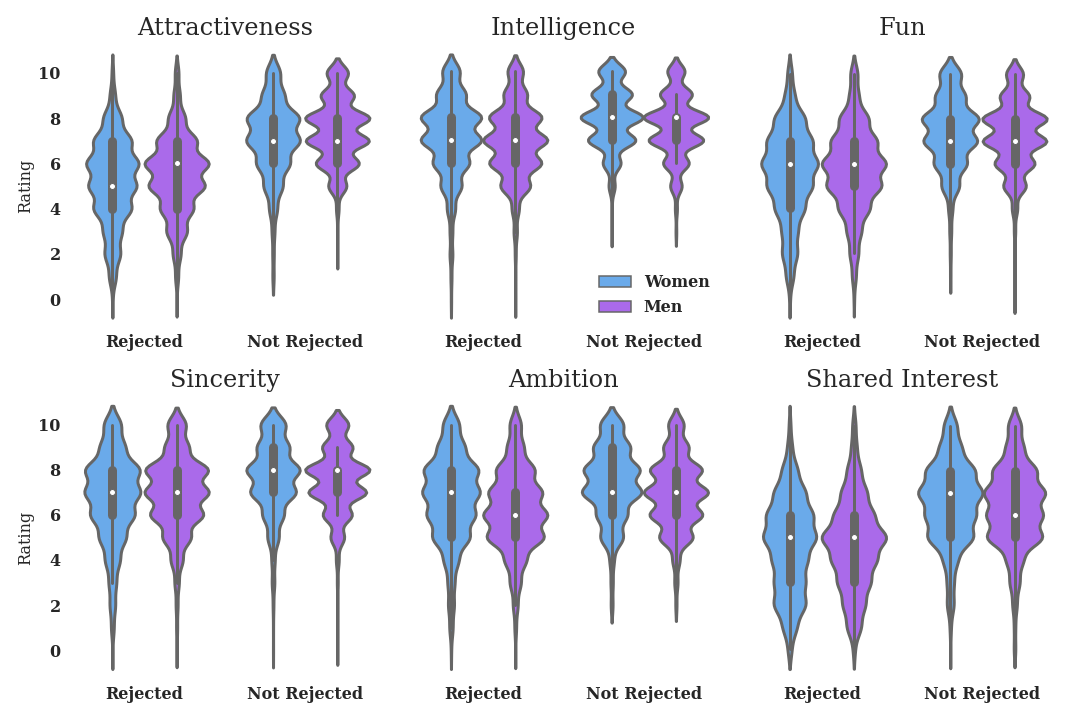
\includegraphics[scale=.375]{project/figures/fig_rejection.png}
\caption{Attribute-Distributions of Rejected and Non-Rejected Partners by Gender}
\label{fig:rejection}
\small Participants rated six attributes of their partner on a scale 1 (awful) to 10 (great). The figure shows the distribution of the ratings by men and women for the respective attribute of the rejected and non-rejected partners. The white dot denotes the median value of each distribution. 
\end{figure}

\textbf{Evaluation.} Indicated by the median displacement in the distribution, the data implies that men reject more attractive women, whereas there no noteworthy difference in the other attributes except women seem to reject more ambitious men. 
We note a distribution shift towards higher ratings for non-rejected partners across all six attributes for both genders. This is expected as higher perceived positive attributes should be positively correlated with a successful first impression.
%Both men and women go for more attractive, intelligent or fun partners. 
%Note, that we analyzed perceived attributes reported by the actual participants of the date and their decision accordingly. It might therefore be reasonable that higher perceived positive attributes are correlated with a successful first impression.
In case of non-rejected partners, we cannot see major differences across the attributes between the genders, except a small median shift in shared interest for women, indicating that women seem to prefer shared interests more than men. 

%Note, that we analyzed perceived attributes reported by the actual participants of the date and their decision accordingly. It might therefore be reasonable that higher perceived positive attributes are correlated with a successful first impression.
 
\section{Predictive Factors of a Successful Impression} \label{sec:factors_impress}
%In the following we will conduct two separate analysis. At first we are focusing on the predictive power of various features on a successful first impression to answer which seem to be influential and if those differ between men and women. Thereafter, we are focusing on a successful first impression based on the participants self-image to see if someones self-perception has any influence of the decision of the partner.  

To address what features seem to be influential, we are applying a logistic regression using the final decision of the participant as a target variable (\autoref{tab:feature_1}). 
We are concluding this analysis by running multiple classification algorithms, analysing the actual predictive power of those features (\autoref{tab:classif_1}).  

\textbf{Data Preparation.} We are using the participant's ratings from \autoref{sec:rejection} as features. 
Moreover, we include likeability, the general perceived expected success rate, the perceived likelihood that the partner will decide for a second date and if both partners have the same ethnicity. 
After extracting features, rows including missing values are deleted and the set is split by genders having 3623 and 3685 examples for women and men, respectively. Both are then randomly split into 70\%/20\% for training and test, whereas the training is split again into 70\%/30\% for training and validation.

\textbf{Feature Importance.} We can see from \autoref{tab:feature_1} that attractiveness seems to have a high contribution on participants decisions, in accordance with \autoref{fig:rejection} being higher for men. Yet, contrary to it, the analysis indicates that intelligence, sincerity and ambition seems to have a negative effect on the decision for both genders, whereas fun and likeability have a positive one. The ethnic background seem to have no effect on women whereas it negatively effects men's decisions. Having too high expectations negatively impacts the decision for men but positive for women. The perceived likelihood actually has a significant positive effect for men but not for women.  

\textbf{Predictive Power.} The features seem to have predictive power across multiple classifiers (see \autoref{tab:classif_1}). 
We are choosing the simplicity of the LR over the SVM, having a final test accuracy of $74\%/78\%$ for men and women. The model for women performs significantly better and seems more robust when comparing precision and accuracy values. 
%Still, we want to highlight the dataset bias in term of location (U.S.), the time-frame for making an impression (4 minutes) as well as the time it was reported (2002-2004). We highly doubt its general effectiveness.   
%Only global feature attribution, no local explanation. 
Still, we highly doubt the general effectiveness of both models due to dataset bias and age described in \autoref{sec:ethics}.

%%%
\begin{figure}
\begin{floatrow}
\capbtabbox{%
     \begin{tabular}{lrr}
          \toprule
          \multicolumn{3}{c}{\small Logistic Regression}\\
            Variable & Coef. \male & Coef. \female \\
          \midrule
            Attractive & $0.41^{*}$  & $0.18^{*}$ \\
            Sincere & $-0.41^{*}$ & $-0.20^{*}$	\\
            Intelligent & $-0.28^{*}$ & $-0.28^{*}$	\\
            Fun & $0.12^{*}$ & $0.15^{*}$ \\
            Likeable & $0.56^{*}$ & $0.42^{*}$ \\
            Shared Interest & $0.13^{*}$ & $0.13^{*}$ \\
            Ambitious & $-0.23^{*}$ & $-0.21^{*}$ \\
            Same Ethnicity & $-0.50^{*}$ & $-0.15^{\phantom{*}}$ \\
            Perc. Exp. Success & $-0.29^{*}$ & $0.17^{*}$ \\
            Perc. Likelihood & $0.13^{*}$ & $0.04^{\phantom{*}}$ \\
          \bottomrule
    \end{tabular}
}{%
  \caption{Feature importance}%
  \label{tab:feature_1}
}
\capbtabbox{%
     \begin{tabular}{lcccc}
      \toprule
      \multicolumn{5}{c}{\small Validation Set}\\
        Model  & Acc. \male & Prec. \male & Acc. \female & Prec. \female \\
      \midrule
        LR & 76.6 & 76.8 & 77.6 &  72.5 \\ 
        NB & 73.7 & 72.0 & 72.3 &  60.9\\
        SVM & 77.4 & 77.4 & 76.9 &  72.8\\
        RF & 76.6 & 75.8 & 76.6 &  71.1 \\
        MLP & 70.8 & 64.2 & 73.1 &  77.1 \\
        KNN & 74.3 & 72.7 & 74.7 &  68.6 \\
        \midrule
        \multicolumn{5}{c}{\small Test Set}\\   
        LR & 74.0 & 64.0 & 78.0 &  72.0 \\
      \bottomrule
      \end{tabular}
}{%
  \caption{Classification}%
  \label{tab:classif_1}
}
\end{floatrow}
\vspace{0.3cm}
\small \autoref{tab:feature_1} shows multiple coefficients of features used as predictors for the decision of the participant with a significance level $\alpha$ of $1\%$ (denoted by *). Those are then compared on multiple classifiers (Accuracy/Precision in $\%$) in \autoref{tab:classif_1}: Logistic Regression (LR.), Naives Bayes (NB), Support Vector Machine (SVM), Random Forest (RF), Multi-Layer-Perceptron (MLP) as well as K-Nearest-Neighbors (KNN). 
\end{figure}

\section{Ethics} \label{sec:ethics}
We do not recommend using our models for practical purposes. The data was compiled between 2002-2004 in the United States and might therefore be biased towards the specific society and observations. Findings might not be transferable to other societies/cultures \cite{shiota2010love}. Further, a lot has changed in the perception of men as well as women in the last 20 years, including cultural shifts such as the MeToo movement \cite{hillstrom2018metoo}. 
%The used dataset is biased in terms of its location as well as time-frame of meetings being four minutes. The dataset used is relatively old, not taking cultural shifts and new perception of men and women into account. 
Our reported models are focusing on the global feature attribution, there is no local explanation. A final decision on a second date is highly individual and shouldn't be judged by a small set of features, being very discriminating in their approach. 
Moreover, our reported models seems to be unfair in terms of its explanatory value between men and women. As we can see in \autoref{tab:classif_1}, the model for women performs better than for men. We either have another dataset bias or it is not comprehensive enough in the decision making for men. 
All in all we emphasize to take our results with a certain degree of scepticism and critical thinking, not to heart. 

\section{Conclusion}
The data indicated clear overlaps and distinctions between interest of men and women as well as women being seemingly more selective than men. Men and women reject less partners rated higher on all attributes. 
%Intelligence and ambition seem to be less important for a successful first impression after 4 minutes. 
For a more fine-grained analysis on the decision making, the LR results show that attractiveness, being funny, likeability and shared interests are the most important markers for predicting a first positive impression.  
%We already encouraged to take our results with a degree of scepticism and critical thinking. 
We do not recommend using our models in practice due to dataset bias and fairness issues between men and women.
%and encourage to take our results with a degree of scepticism and critical thinking.

\bibliographystyle{plain}
\bibliography{bibliography_strings,bibliography_custom}

%\section{Appendix}

\end{document}
